\chapter{Application}

The listed algorithms have their theoretical benefits, but they might not be good for real issues. The numeric obstacles require the trade-offs between robustness, stability, and calculation time. The computer memory has limited capacity; systems discretization adds the plant errors. We considered the examples do not have a physical reference system. Now, we try to apply the algorithms on the more ''real'' plant and see the problems that occur. 



	\begin{exam}
		 We consider a dynamical system, which describes a flexible satellite. As known from \cite{SchRC} the continuous-time transfer function has the form  
		\begin{align}
		G(s) = \frac{.036(s + 25.28)}{s^2(s^2 + .0396s + 1)}. 
		\end{align}
		As input we choose the torque on first mass, and as output is set the position $\theta_2$. 
		
		Since we are working with discrete time systems, we discretize it for sample time $T_s = 10^{-3}$  and get the state space description 
		\begin{align}
		\label{eq:Appl:satellite_sys}
		\left( \begin{array}{c | c}
		A & B \\ \hline C & D
		\end{array}\right) = 
		\left(\begin{array}{c c c c | c}
	    1.000  &  0.005  &  0.000  &  0.000 & 1.047\cdot 10^{-13}\\
		0  &  1.000  &  0.001  &  0.000 & 8.333\cdot 10^{-11}\\
		0  &       0  &  1.000  &  0.001 & 2.5\cdot 10^{-7}\\
		0  &       0  & -0.001  &  1.000 & 5\cdot 10^{-4}\\ \hline
        0.362 & 0.072&  0 & 0 & 0
		\end{array}\right). 
	\end{align}
	\end{exam}

In this example, the matrix $D$ is zero, what makes our algorithms not applicable. 
Moreover, the  $D$-part's neglecting is typical: the system output must mostly image the system state and not the known input we send. 

To see more precisely, the input update rule has the form 
\begin{align}
y(t) = C x(t) = C(A x(t) + B u(t)) \text{ for } t = 0, 1,2, \dots, N. 
\end{align}

With other words, the input $u(t)$ begins to impact the output by first iteration, if the matrix $CB$ is not a zero-matrix. That means, that the \textit{relative degree} of the system equals 1. We define it mathematically precise: 
\begin{defi}
	The relative degree of the system $(A, B, C, D)$ is 0 if $D \neq 0$. For $D = 0$ it is the smallest integer $k$ for which $	C A^{k-1} B \neq 0$.
\end{defi} 
Let us denote it with $k^*$. Then the new system we consider can be written as 
\begin{align}
x(t+1) &= A x(t) + B u(t), \\
y(t) &= C x(t) + C A^{k^*} B u(t),  \text{ for } t = k^*, k^* + 1, \dots N. 
\end{align}

We need to put the first iterations away and define a new initial condition $x(k^*)$. The start input condition is then $u(k^*)$. 

For new system all the requirements we considered are satisfied. However, we do not get a better solution for $t = 0, 1, \dots, k^\star - 1$. 

%TODO: change the example style 
\begin{example}[continued]
	
\textit{For our system the relative degree is 1, as }
	\begin{align}
	CB = 6.038\cdot 10^{-12} \neq 0. 
	\end{align}
	
\textit{We calculate the solution with LQR. Result is illustrated in Figure \ref{img:Appl:Sat_LQR}.}
	
	\begin{figure}[ht]
		\centering
		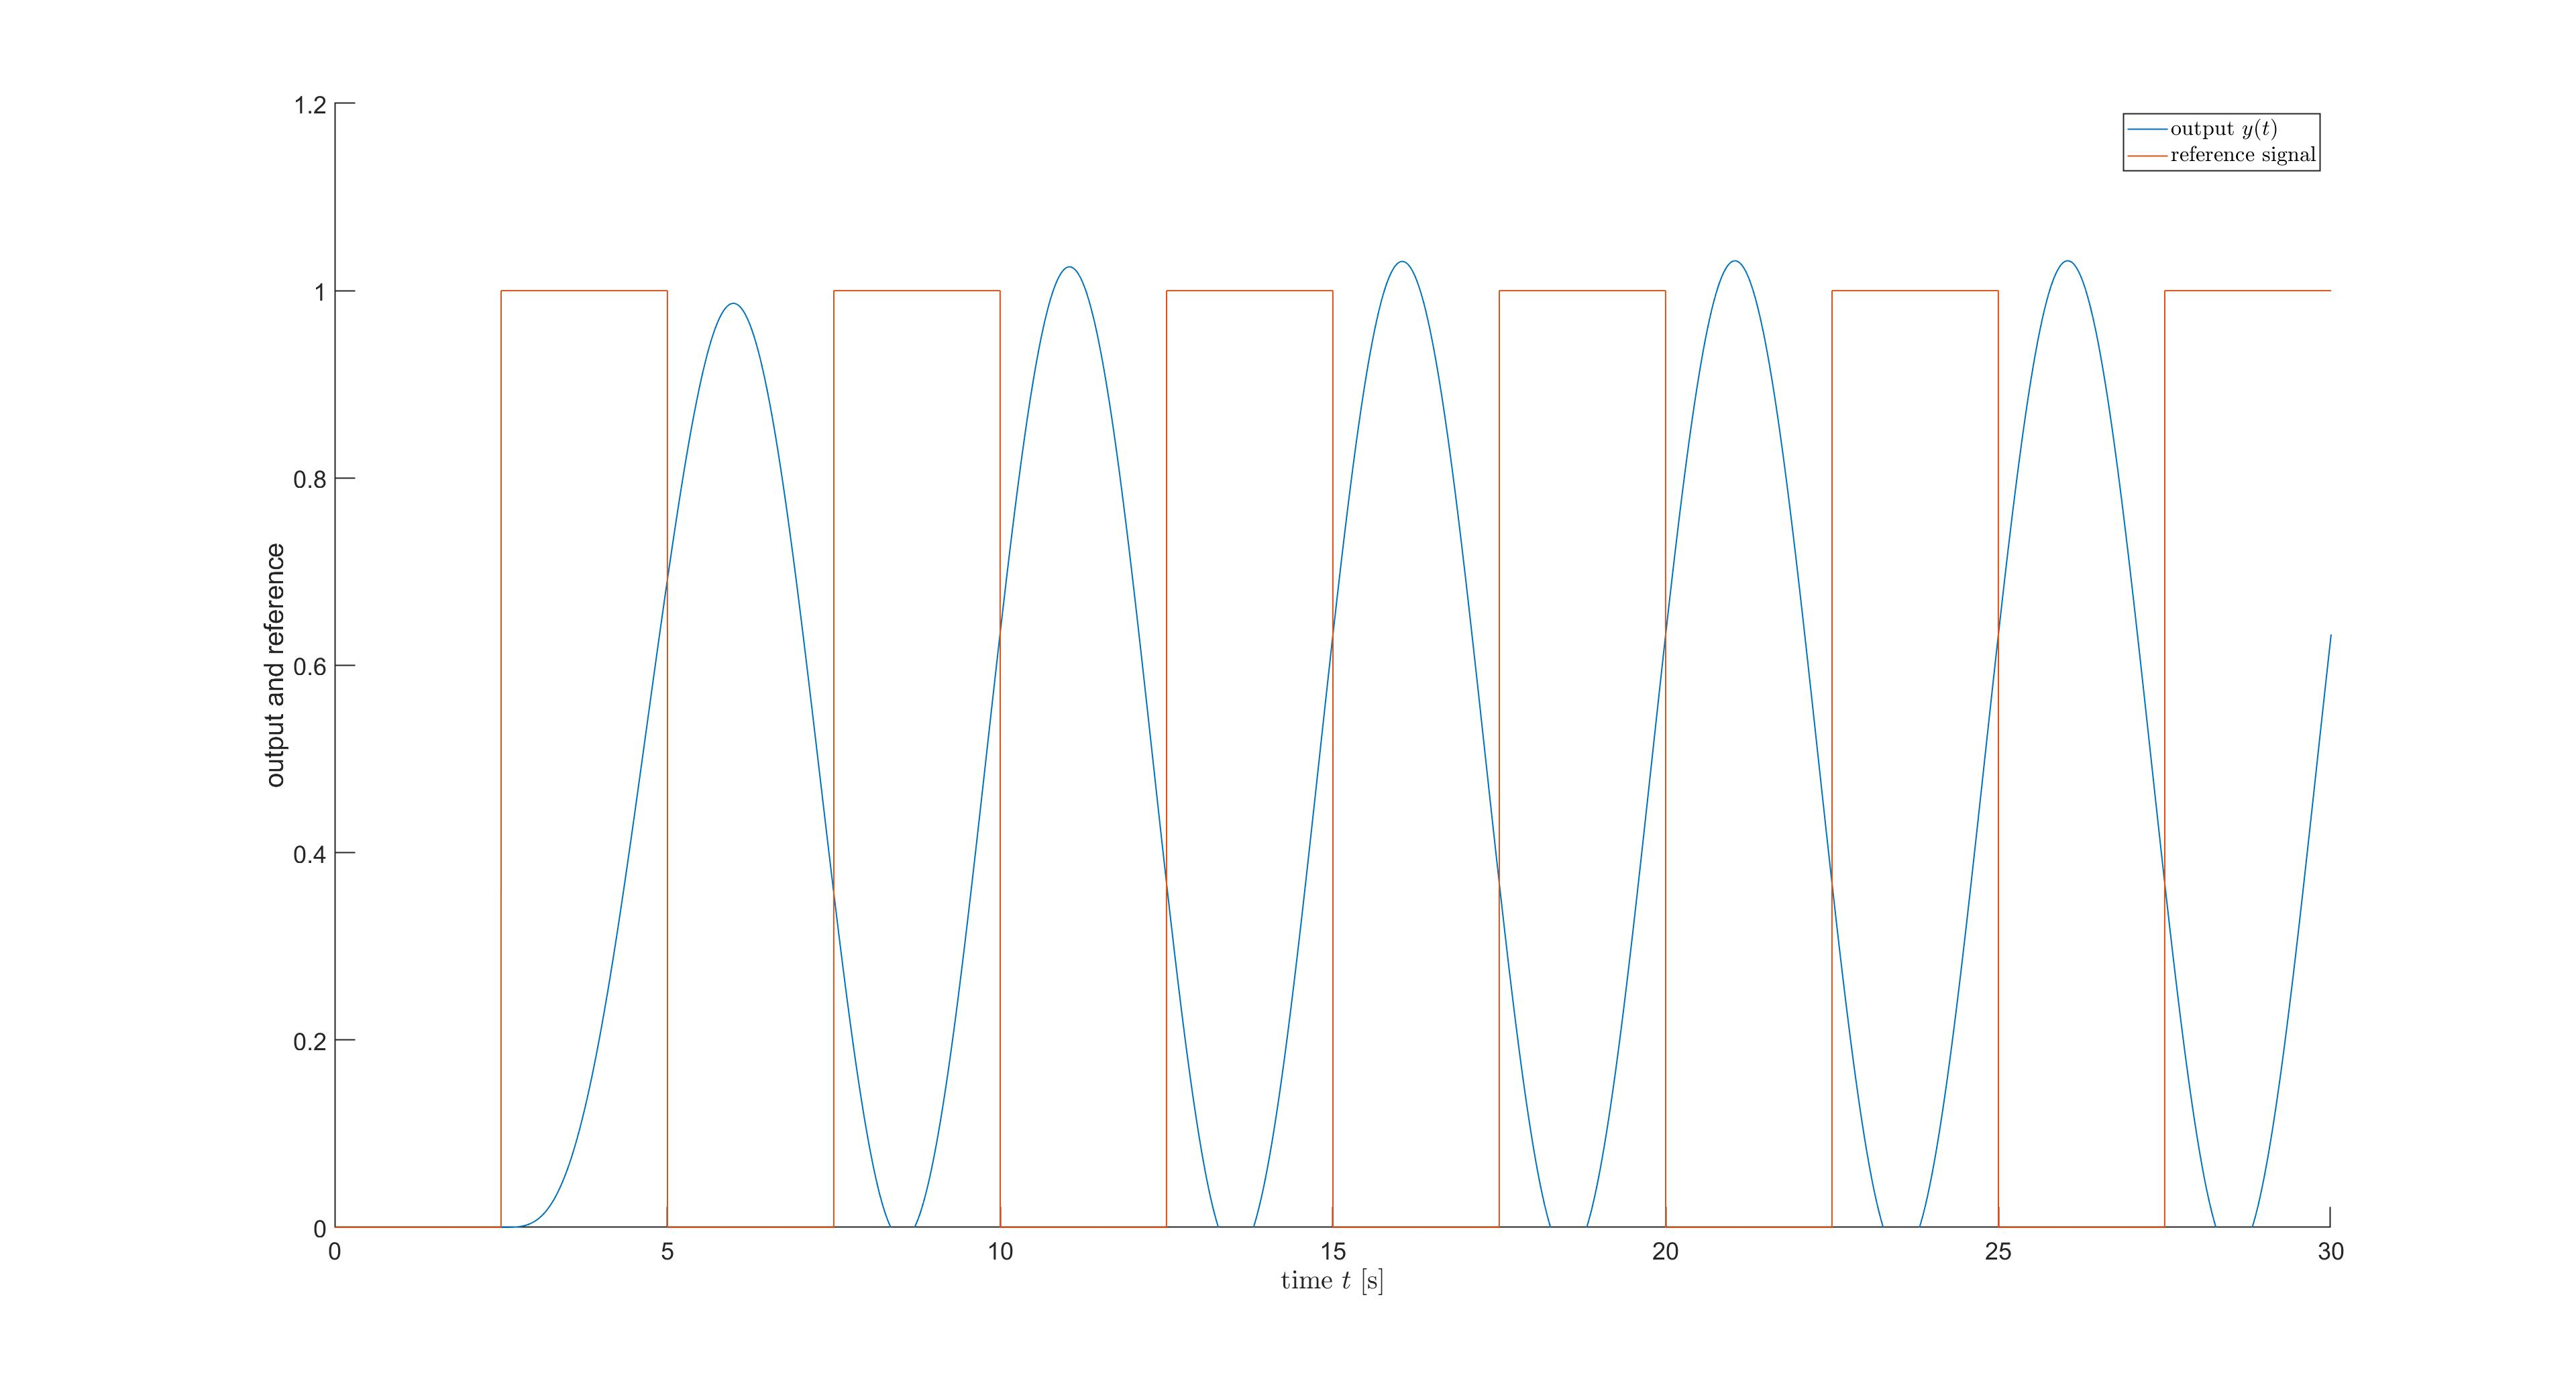
\includegraphics[width=\textwidth]{fig/Ex3_LQR.jpg}
		\caption{LQR Solution for the system \eqref{eq:Appl:satellite_sys}}
		\label{img:Appl:Sat_LQR}
	\end{figure}
	
\textit{It looks like something we can improve. However, for $Ts = 10^{-3}$s we get $N = 10^3$ time steps even for one iteration second. The matrix $G$ has  $10^9$ elements and can not easily be handled.}
\end{example}

	In example \ref{ex:ILC:IAcrushes} the Inverse Model Algorithm is not applicable even for $N = 40$. 
	That means, we need a trade off between the time horizon and robustness.
	However, for real problems the sample times are mostly small, and hence even for one second of the simulation we get huge number for time horizon. Already for SISO system the matrix $G$ will have $N^2$ elements. Our algorithms become unusable for casual applications since they need vast masses of memory.	
		
	We solve this problem by application the algorithms iterative, for smaller number of time steps. We only need to adapt the initial input condition and the reference signal: we split them in $N_{max}/N$ parts, and take each iteration the next one. Here $N_{\max}$ is the number of time steps in total, and $N$ is the number of time steps we put into the algorithms .
	
	The choice of $N$ is than another design  decision to be made. It must be not too large, since a used algorithm can diverge, if it is too small, we probably will need more iterations in total. 
	

\begin{example}[contined]
\textit{Let us use the Steepest descent algorithm, and choose put each time $N =100$ elements into the algorithm. 
The result is depicted in the Figure \ref{img:Appl:Sat_SDA} We can see, that steepest descent algorithm converges very fast to tracking value, and even for 20 iterations we get perfect tracking. 
}
	\begin{figure}[ht]
	\centering
	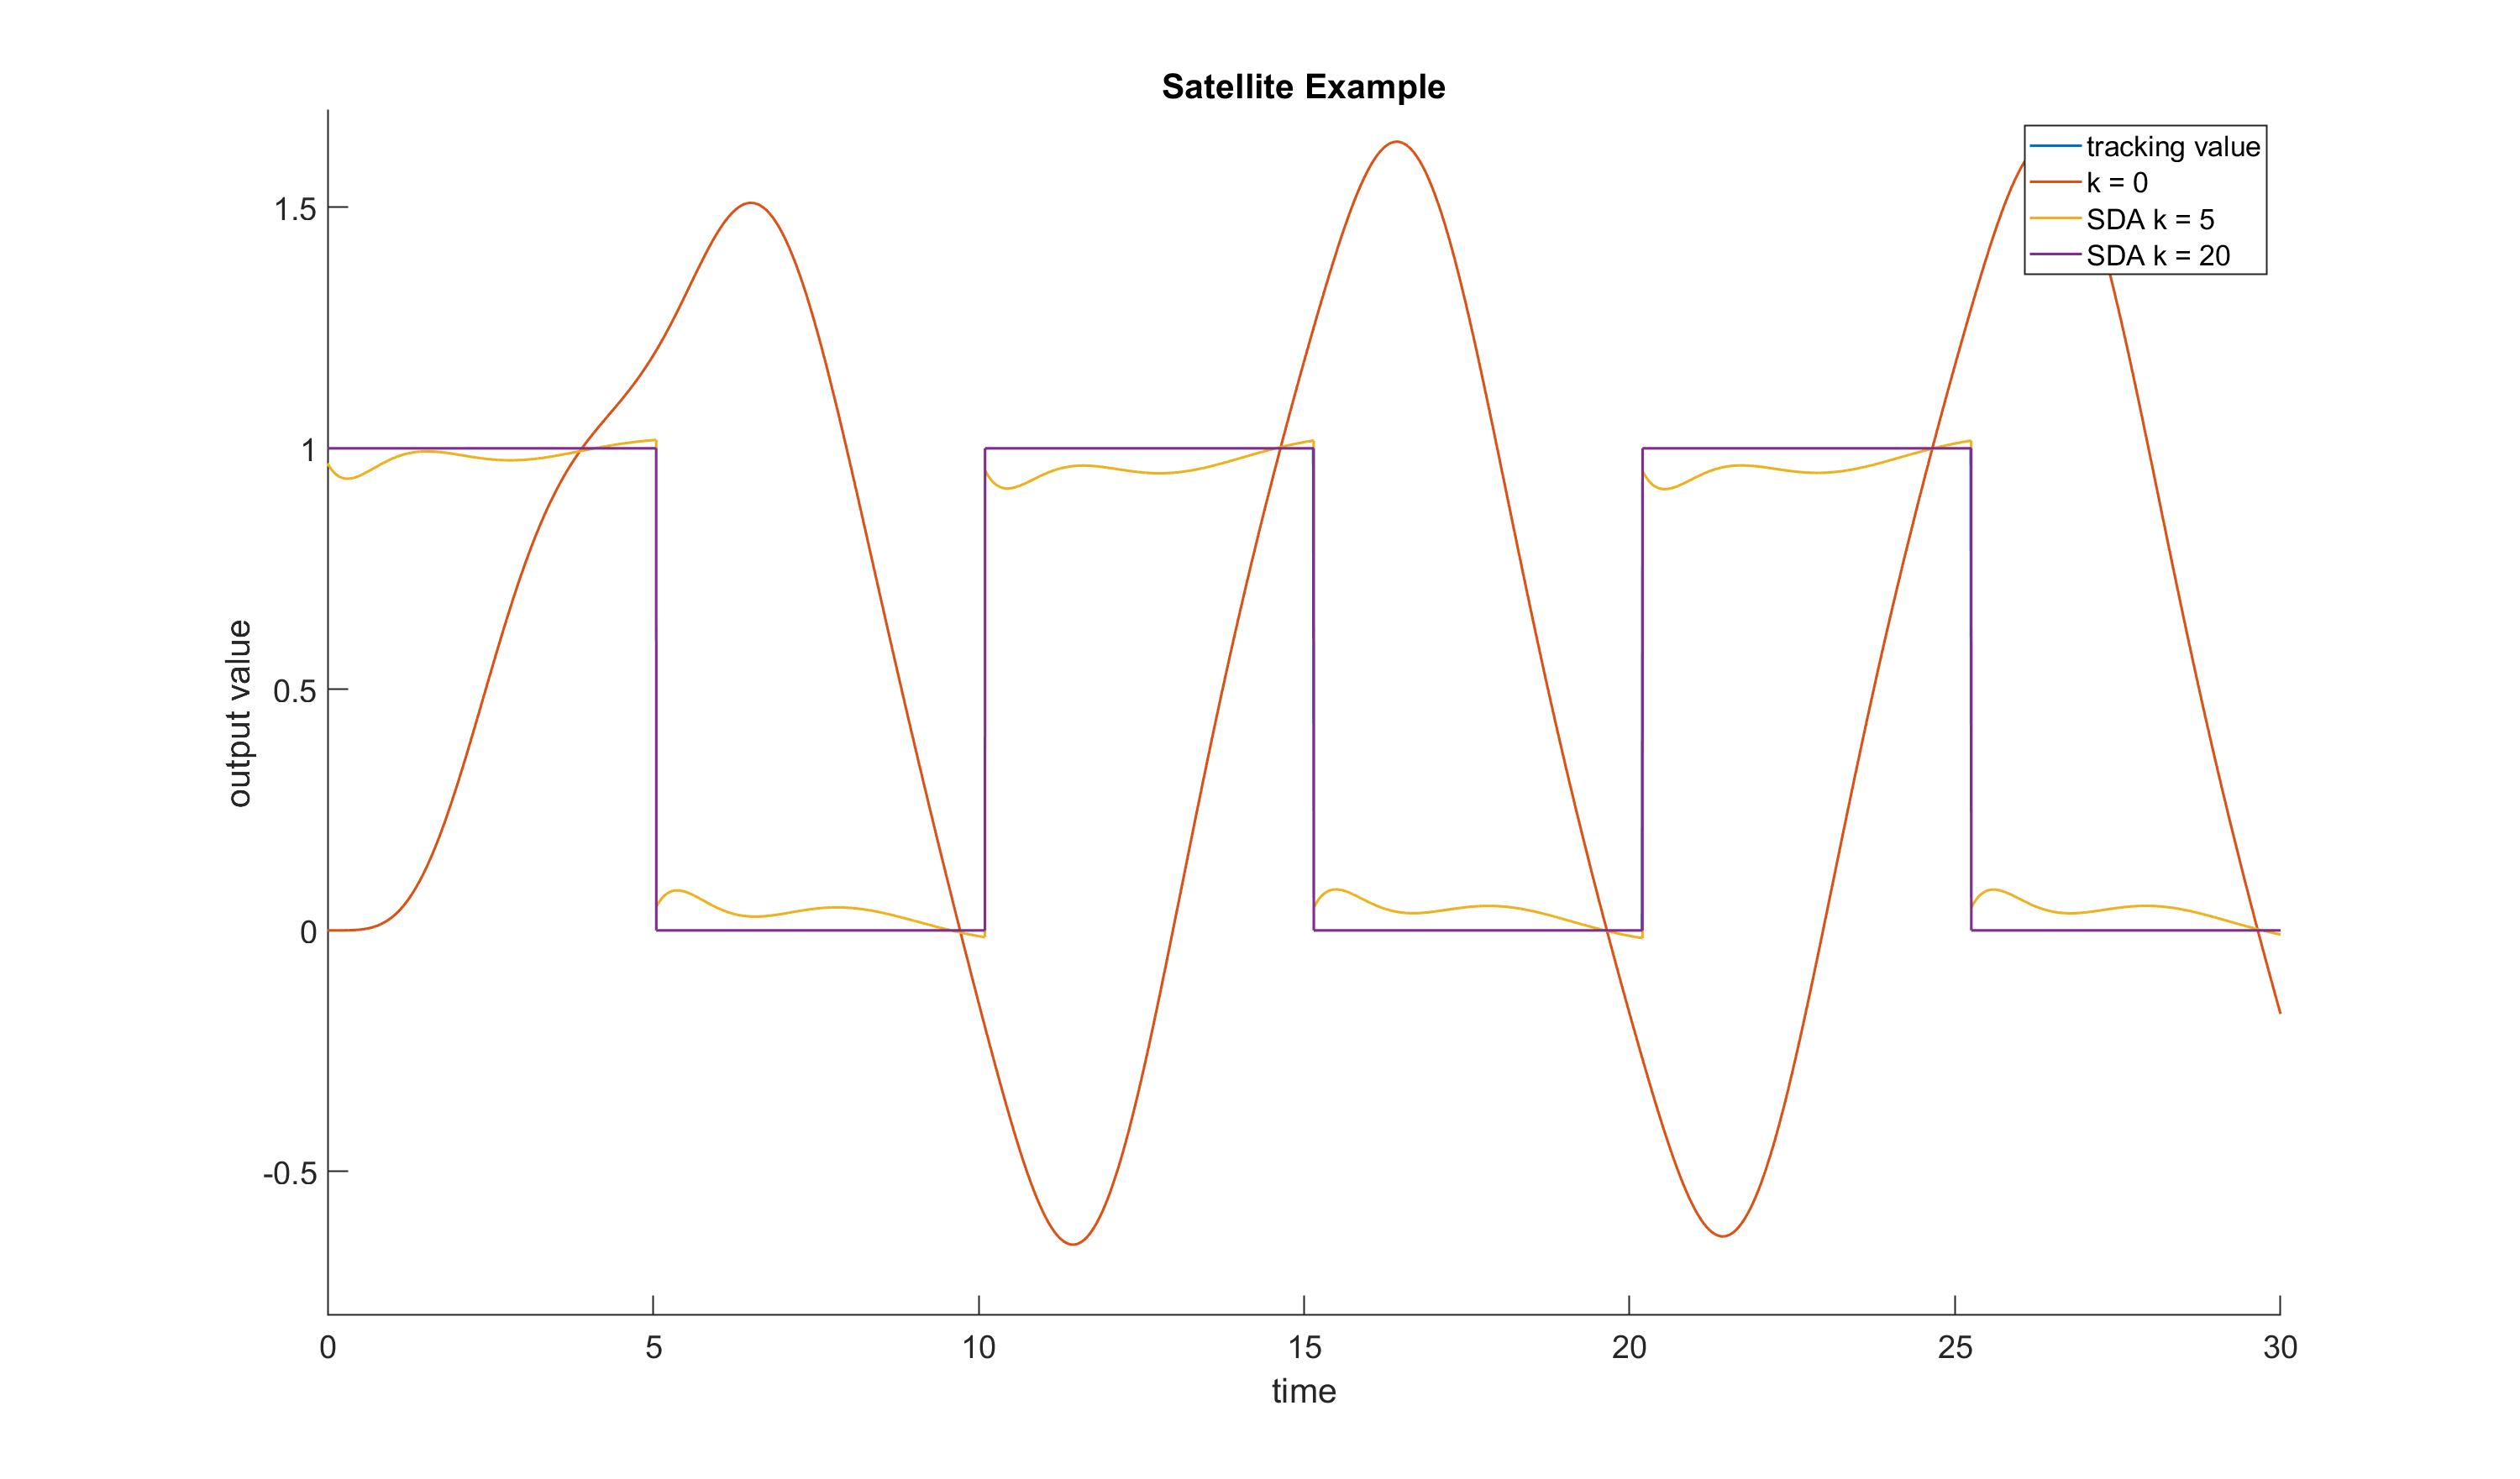
\includegraphics[width=\textwidth]{fig/Satellite_SDA.jpg}
	\caption{LQR Solution for the system \eqref{eq:Appl:satellite_sys}}
	\label{img:Appl:Sat_SDA}
\end{figure}



\end{example}    

	
	
	